\documentclass[10pt]{IEEEtran}
\pdfoutput=1

\usepackage{graphicx}
\usepackage{hyperref}
\usepackage[utf8]{inputenc}
\usepackage{listings}
\usepackage[table]{xcolor}
\usepackage{pdfpages}

\hypersetup{colorlinks=true,citecolor=[rgb]{0,0.4,0}}


\title{Predictive Beer Analytics}
\author{Joshua Weinstein, Jim Sundkvist, Marek Kühn}

\begin{document}
\maketitle

\begin{abstract}
This project aims to apply various concepts of Python programming as well as data mining and processing.
Based on a large amount of user and beer data, the application uses varying techniques including data mining, natural language processing, and color analysis to predict user-defined beers' desirability in the world through a web application. 
\end{abstract}

\section{Introduction}

The Predictive Beer Analytics project has been initiated in the Fall of 2014 as a part of "\textit{Data Mining Using Python}" course at Denmark Technical University. Its purpose is not only exercise the study material, but also to give users some useful, informative results. To satisfy this, we used our previous experience with web development and created a lightweight web-service with visual representations of the results. The users can design their own beer by defining its style, alcohol by volume, keywords and dominant label color. This information is then used to generate a desirability map (ref).

The application to retrieve and analyse data along with our web application (without the database) can be found on our GitHub account. The web-service can be run locally with an installation of \href{https://www.djangoproject.com/}{Django}, \href{http://www.mysql.com/}{MySQL}, and a copy of the database.

\section{Data mining}
Being the main aspect of any data mining project, retrieving the data, and a lot of it, is the first course of action. All data used by Predictive Beer Analytics was gathered through the \href{https://untappd.com/api/docs}{Untappd API}, a beer review website which provides access to the data it collects. Unfortunately, the service limited our access to their data to 100 calls an hour. This significantly increased the amount of time required to gather data. The script, \texttt{untappd.py} provides data structures to store Untappd data as well as uses the \textit{Requests} module to make calls to Untappd's servers. Due to the available requests through the API service, it was necessary to first retrieve a list of active users and then later use their username to gather information about beer they have reviewed in the past. Over the course of roughly two weeks of mining, a reasonable amount of information was stored. Seen in Figure \ref{fig:dataQuantity}, over 200.000 user reviews are used to predict the desirability of a beer based on location. To keep this information up-to-date, \texttt{dataQuantity.py} script has been included in the library. 

\begin{figure}[h]
  \centering
  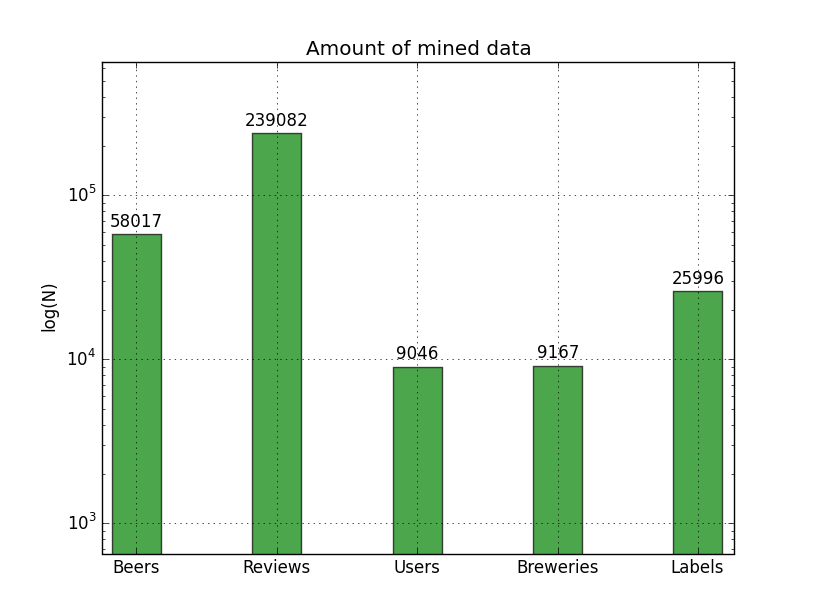
\includegraphics[width=\columnwidth]{./graphics/quantity.png}
  \caption{Amount of used data (by the time of presentation)}
  \label{fig:dataQuantity}
\end{figure}

After data has been gathered, updated, and normalized with methods in the main script \texttt{predictiveBeerAnalytics.py}, it is split up into users and beers where users contain a location, using the \href{https://developers.google.com/maps/documentation/geocoding/}{Google Geocoding API}, and their ratings and beers are composed of descriptive keywords, alcohol content, label's url, style, and other unused information. These are then used in conjunction with other scripts we have written to analyse label colors, determine keywords from descriptions, find relationships between alcohol content and location, and  determining relationships between a user's location and the style of beer they enjoy.

\section{Machine learning}
There are two applications of machine learning: 

\hspace{0.3 cm}
\begin{itemize}
  \item \textbf{Natural language processing}
  \item \textbf{Image color analysis}
\end{itemize}
\hspace{0.3 cm}

With its extraordinary lexical resources and easy-to-use interface, \textbf{Natural Language Toolkit} (\href{http://www.nltk.org/}{NLTK}) was an easy choice. It is used to tokenize the sentence in order to classify the words according to its type. After various filtering (usage threshold, invalid characters etc.), we calculate the average rating of each keyword. The best, worst and the most used keywords are presented on the website. The relevance of the results is to be discussed later. The actual \textbf{keyword extraction} function is defined in \texttt{keywordExtractor.py}, making it easy to reuse in other projects. It is possible to introduce regular expressions in order to improve the keyword recognition, but the results are reasonable even without using it.

While thinking about all aspects that can possibly affect the beer desirability, we introduced also the visual point of view. We have no information about the color of the bottle. Nevertheless, more than half of the beers from untappd have a link to the beer label picture attached. All we had to do is determine how the beers are rated in relation to the label color. The \textbf{dominant colors clustering} is done with \href{http://scikit-learn.org/stable/modules/classes.html#module-sklearn.cluster}{sklearn.cluster} module, built on \href{http://www.numpy.org/}{NumPy}, \href{http://scipy.org/}{SciPy}, and \href{http://matplotlib.org/}{matplotlib}, well-known open-source libraries. All of which are also used regularly in other context in this project. Currently, we use \textbf{K-means clustering} to determine five of the most used colors in each label. The class responsible for the calculations \texttt{labels.py:Image} is designed such as the parameters like number of clustered colors are easy to change in the future.

To check if the result is correct, we use the clustered colors to rebuild the picture as in the figure \ref{fig:colorClustering}. Since we observed a lot of labels not having rectangular shape, we implemented a \textbf{custom masking algorithm} based on the color differences. It seeks a border at which certain threshold is overrode and generates numpy.mask. This is covered by \texttt{labels.py:Mask}. 

\begin{figure}[b]
  \centering
  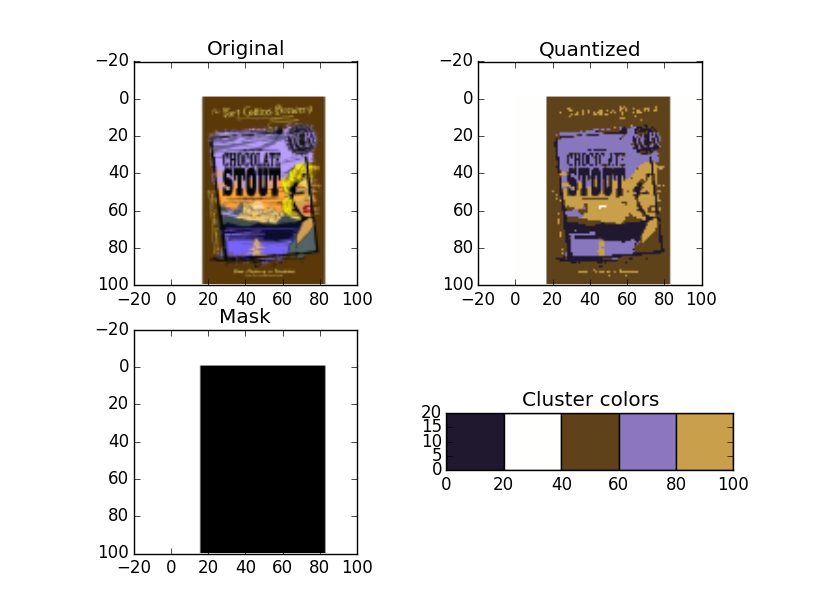
\includegraphics[width=\columnwidth]{./graphics/1.png}
  \caption{Image color clustering}
  \label{fig:colorClustering}
\end{figure}

Having these colors extracted, they need to be associated with ratings. Otherwise there would be no measurable impact on the total beer desirability. We couldn't match those color directly to the user input, because that way its rating would have to be calculated  every time the request is made, which is not acceptable given the amount of data. So we come up with a solution by using template color palette. It serves as a fixed categorizing root. None of the available functions were suitable for comparing the RGB values of the colors, so we designed our own classification algorithm. It uses the well-known euclidean distance formula to determine which color from the template color palette is the closest. However, simple distance in RGB colorspace doesn't correspond to human perception. A change of one parameter results in much more different color than the same change distributed between multiple parameters. It was possible to overcome this by converting the colors to YUV colorspace (Fig. \ref{fig:colorspace}), which takes human perception into account, making the response more or less linear. 


\begin{figure}[t]
  \centering
  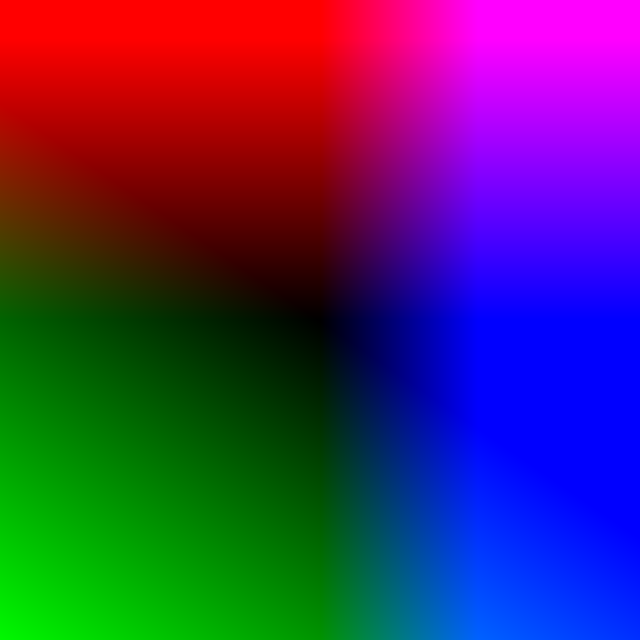
\includegraphics[width=6cm]{./graphics/YUV.png}
  \caption{YUV linear colorspace sample for Y = 0}
  \label{fig:colorspace}
\end{figure}

\section{Web application}

The web application uses one of the most popular Python frameworks - Django. This allowed us to create elegant web application while still being able to focus on the server-side python scripts rather than web-design.

The web-design and structure of the web application is pretty straight forward:
A landing page that serves as a portal and first encounter information of the web applications functionality.
A prediction page where the core of PBA is preformed.
The user can fill in data that would reflect their beer and check where it would do well with a histogram.
A Description page where a off the bat ranking of the processed words are presented.
Here it is also possible to search for a specific word.
The result will be a list of similar words and their ranking starting form the highest rating.
A color page where the user can see the rankings off colors used in beer labels.
An about page where we tell the story and information about Predictive Beer Analytics.
And last a map page where we showcase some predefined results from the predictor.

Django uses the MVC architecture. So the Project has a data model, representing our processed data was created.
A single view file that contains all (as the size of the Web application was not large enough to warrant separation of concerns in our eyes) application level functionality. And templates which uses css and javascript to make a smoother appearance.
Bootstrap was used to speed up the styling in this regard. All templates extends the base.html template which
acts as a master page.

The data that the web application uses are stored in a MySQL database.
The data itself is generated from the data mining scripts and saved to the web applications database by importing them as a scv file.
The web application uses Django's database-abstraction API to perform the basic CRUD functionality to the data model SE FIGURE ?.
 
When it comes to security Django has some great features that will bring about basic security with minimum effort.
Django's database-abstraction API automatically sanitizes any input so SQL-injection is not a problem.
Cross-site-scripting is dealt with by using csrf tokens.
Responses automatically has csrf tokens inside so when doing POST you only need to add it.
In a Form simply having  takes care of the problem.
Django also have some predefined user authentication and authorization functionality.
In the web application we do not use any access control so this part is unnecessary until a time arrive when we do need it.

The decision to use these technologies is pretty straight forward:
The technologies were familiar, well used and documented, and easy to use.
This lead to quite a fast development of the PBA GUI.



\section{Discussion}

Keywords - Regular expression.

Hardcoded web color palette

\section{Further development}
Collecting data

Machine learning

Website

Including brewery information


\section{Results}
At the beginning of Predictive Beer Analytics, our goal was to find relationships between the alcohol content or style of a beer and the location of a user's rating to determine what areas enjoy the most. As the project progressed, ambitions rose and we wanted to see if the color of the label or the description of beers made a significant impact on the desirability of a beer. Using \texttt{PBAMap.py}, \texttt{keywordClassifier.py} we are able to graphically visualize the effects of specific words, alcohol content, and beer style on a user's rating. Figure \ref{fig:abvcomp} shows the consistent and seemingly global idea that people typically enjoy stronger beers. While there is a clear correlation between user reviews and and a beer's alcohol content, the type of beers an area likes are typically varied and relatively unpredictable. Though it does seem that the United States enjoys IPAs more than ciders and fruitier beers.

It was also interesting to see that certain words used in a beer's description had a large impact on a user's review of the beer. For example, beer descriptions containing words like "inexpensive", "alcohol-free", and "grandma" all had an average rating of below three out of five stars. Whereas "sought-after", "chocolate-covered", and "fabled" all had ratings above four stars.

\begin{figure}[t]
  \centering
  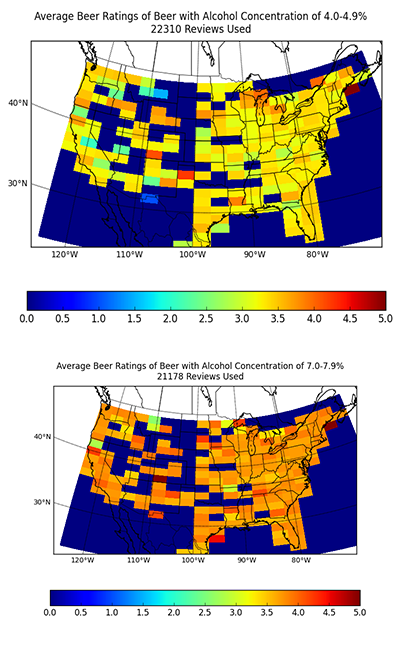
\includegraphics[width=6cm]{./graphics/abvComp.png}
  \caption{Comparison of average beer ratings in US based on alcohol content}
  \label{fig:abvcomp}
\end{figure}

\section{Discussion}


\section{Conclusion}


\bibliographystyle{IEEEtran}
\bibliography{lyngby}


\clearpage
\onecolumn
\appendices
\section{Code listings}

\definecolor{darkgreen}{rgb}{0, 0.4, 0}
\lstset{language=Python,
  numbers=left,
  frame=bottomline,
  basicstyle=\scriptsize,
  identifierstyle=\color{blue},
  keywordstyle=\bfseries,
  commentstyle=\color{darkgreen},
  stringstyle=\color{red},
  literate={Ö}{{\"O}}1 {é}{{\'e}}1 {Å}{{\AA}}1,
}
\lstlistoflistings

\label{listing:PBA}\lstinputlisting{../machine_learning/lib/predictiveBeerAnalytics.py}

\label{listing:Untappd}\lstinputlisting{../machine_learning/lib/untappd.py}

\label{listing:keywordExtractor}\lstinputlisting{../machine_learning/lib/keywordExtractor.py}

\label{listing:keywordClassifier}\lstinputlisting{../machine_learning/lib/keywordClassifier.py}

\label{listing:dataPoints}\lstinputlisting{../machine_learning/lib/dataPoints.py}

\label{listing:PBAMap}\lstinputlisting{../machine_learning/lib/PBAMap.py}

\label{listing:labels}\lstinputlisting{../machine_learning/lib/labels.py}

\label{listing:fileReader}\lstinputlisting{../machine_learning/lib/fileReader.py}

\label{listing:dataQuantity}\lstinputlisting{../machine_learning/lib/dataQuantity.py}


\newpage
\section{Automatic generation of documentation}

Demontration using epydoc:
\begin{verbatim}
epydoc --pdf -o /home/fnielsen/tmp/epydoc/ --name RBBase wikipedia/api.py
\end{verbatim}
This example does not use \verb!brede_str_nmf! but another more
well-documented module called {\tt api.py} that are used to download
material from Wikipedia. 

%\includepdf[pages={-}]{/home/fnielsen/tmp/epydoc/api.pdf}

\end{document}
